\documentclass{IIBproject}

\usepackage{setspace}

\usepackage{amssymb,amsmath,amsthm}
\usepackage{units}
\usepackage{cite}
\usepackage{subfigure}
\usepackage{minted}
\usepackage{url}
\usepackage[margin=2.5cm]{geometry}
\usepackage{multirow}
\usepackage{import}

\usepackage[retainorgcmds]{IEEEtrantools}

% required to get proper length monospace underscores
\usepackage[T1]{fontenc}

\DeclareMathOperator*{\argmax}{arg\,max}
\DeclareMathOperator*{\argmin}{arg\,min}

\usepackage{graphicx,ctable,booktabs}
\graphicspath{{figures/}}

\pagestyle{empty}
\onehalfspacing

\begin{document}

% Title Page
\author{Rodrigo Queiro (DOW)}
\title{Machine Learning for Control}
\projectgroup{F}
\maketitle
\thispagestyle{empty}

% Summary
\renewcommand{\abstractname}{Technical Abstract}
\begin{abstract}
  technical abstract\ldots
\end{abstract}
\pagestyle{plain}
\tableofcontents
\newpage

\section{Introduction}

Balancing a unicycle is a very challenging task for a
human rider. Many attempts have been made to achieve this task, using a
variety of models for the action of the rider. Some represent the rider as a
flywheel or pendulum in the coronal plane, allowing direct compensation of
falling to the side\cite{ref:zenkov,ref:murata}, as in
Figure~\ref{fig:murata}. Other use a more realistic (and challenging) model of
a flywheel in the horizontal plane\cite{ref:vos,ref:naveh}, as in
Figures~\ref{fig:naveh_unicycle}, but none of these
have reliably balanced a real unicycle.

\begin{figure}[htbp]
  \begin{center}
    \subfigure[Murata Girl]{
      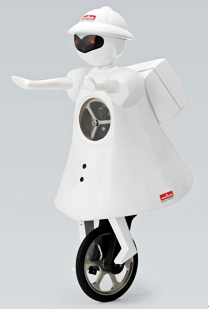
\includegraphics[height=5cm]{figures/murata_girl.jpg}
      \label{fig:murata}
    }
    \subfigure[Naveh's Model]{
      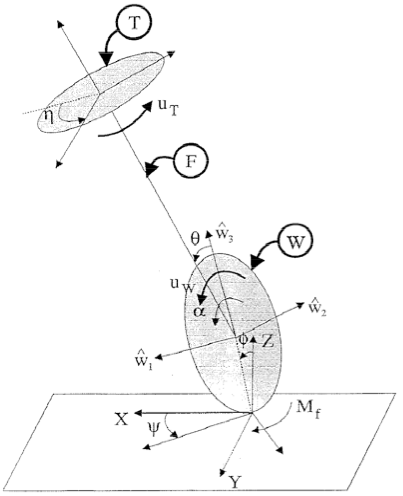
\includegraphics[height=5cm]{figures/naveh_unicycle.png}
      \label{fig:naveh_unicycle}
    }
    \subfigure[2D Problem]{
      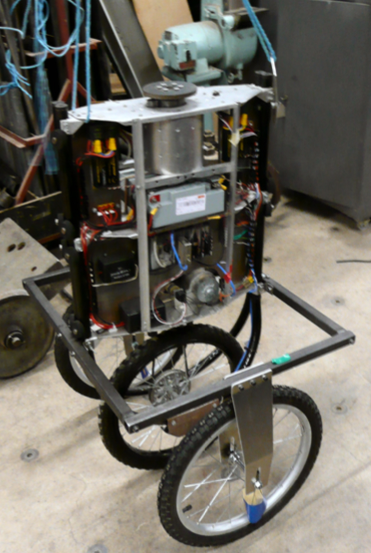
\includegraphics[height=5cm]{figures/forster_unicycle.png}
      \label{fig:forster_unicycle}
    }
    \subfigure[3D Problem]{
      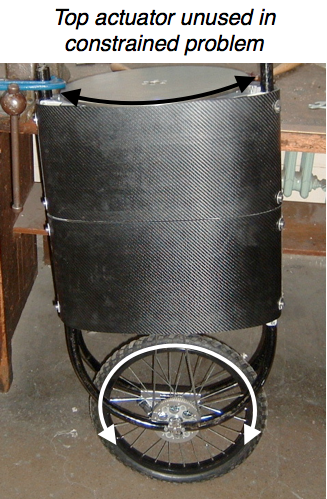
\includegraphics[height=5cm]{figures/3d_unicycle.png}
      \label{fig:3d_unicycle}
    }
    \end{center}
    \caption{Different balance problems}
    \label{fig:unicycles}
    \end{figure}

In 2004/2005 Mellors and Lamb \cite{ref:mellors,ref:lamb} built a robotic
unicycle, shown in Figure~\ref{fig:3d_unicycle}, intending to design a controller to balance it. However, they were
only able to complete the construction of the unicycle. In 2007/2008,
D'Souza-Mathew resumed work, replacing a wheel sensor and attempting to design
a controller. He simplified the problem by removing the ability to fall to the
side, reducing it to 2D dynamic control: the inverted pendulum (from
now on referred to as the \textbf{2D system}). This is shown in
Figure~\ref{fig:forster_unicycle}. He was unable to balance the unicycle due to
hardware problems.

Next, in 2008/2009 Forster analysed the dynamics of both the 2D problem and
the unrestricted 3D unicycle\cite{ref:forster}. Again, hardware problems
prevented him from balancing the 2D system, and although he designed a
controller for the 3D unicycle, it was not even tested in simulation. Given
the simplicity of his approach compared to those of Vos and Naveh
\cite{ref:vos,ref:naveh}, it appears unlikely to work.

One thing all these approaches have in common is that their first step is a
series of simplifying assumptions about the dynamic system. They ignore the
non-linearities like motor dead-zones and wheel friction that are present in
any real-world system, and attempt to design a controller to stabilise the
idealised system. In many cases, this approach is very successful. However,
D'Souza-Mathew and Forster found that their model was invalid since the
unicycle's motor drive didn't react faster enough. Vos and Naveh had to use
complex, approximate techniques to model the unicycle.

An alternative ``intelligent'' approach to control involves learning the
dynamics of the system directly, instead of relying on assumptions and
mechanical analysis. Various methods for this have been used, but many require
prohibitively large amounts of data from the system. One method due to
Rasmussen and Deisenroth, known here as Reinforced Model Learnt Control
(RMLC), achieves unprecedented data efficiency, and has been successfully used
to stabilise a computer simulation of a 3D
unicycle\cite{ref:rasdei08,ref:rasdei11}.

In 2009/2010, McHutchon successfully applied RMLC to the 2D system
\cite{ref:mchutchon}. However, since he had to make significant changes to the
unicycle hardware and software to achieve this, he did not have time to
attempt to balance the 3D unicycle.

The principle objective of this project is to apply RMLC to the unrestricted
3D unicycle. This includes the solution of problems identified by McHutchon,
as well as other problems identified during the project.

\subsection{Division of Labour}

This project was conducted as a joint project between the author and Alan
Douglass. The vast majority of the work was done together, and as such it is
difficult to attribute ideas or components of the system to one or the other.
When only one of us was responsible for a particular component, such as a
particular circuit or module of the code, it is focussed upon in their report,
and the other report will simply refer to it.

Although this may raise difficulties for marking the projects, it was
essential for the actual work. We would never have been able to make such
progress if we had not been able to build on each other's ideas, to spot each
others mistakes and to rely upon another point of view when stuck.

\section{Reinforced Model Learnt Control}

\begin{figure}[htbp]
  \begin{center}
    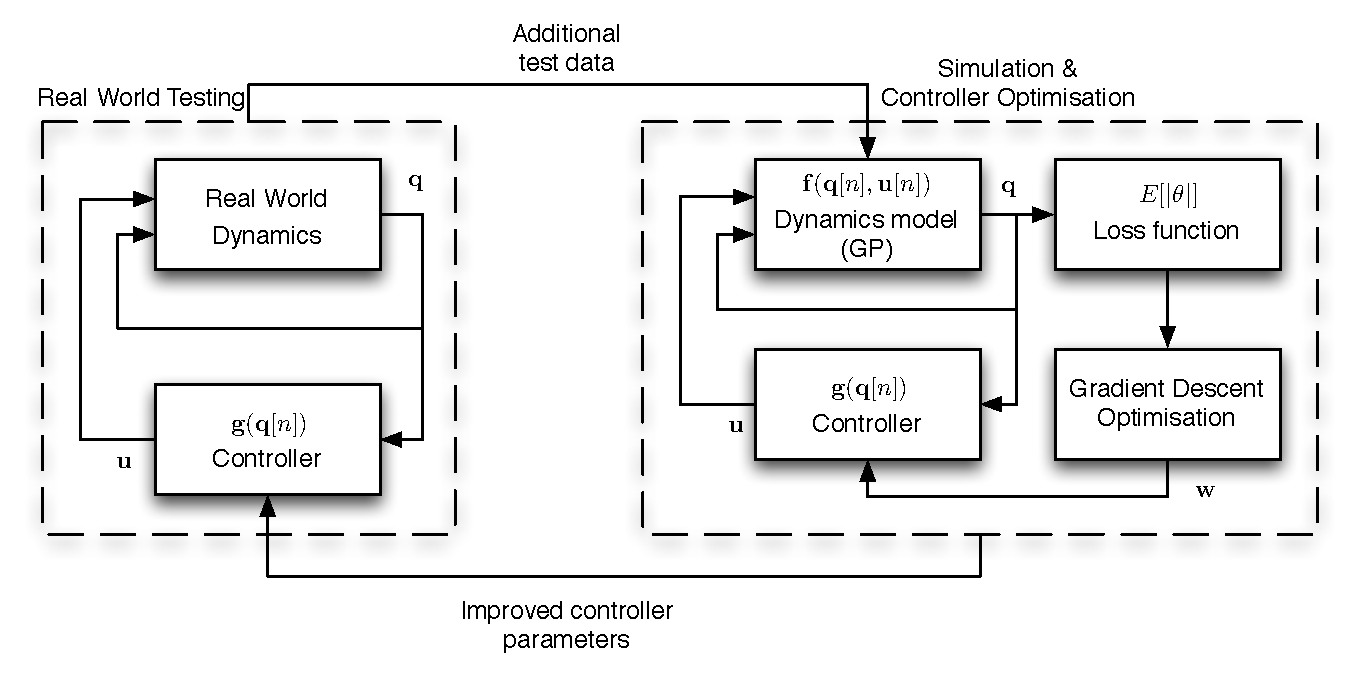
\includegraphics[width=14cm]{figures/GPRMLC.pdf}
    \end{center}
    \caption{Reinforced Model Learnt Control}
    \label{fig:rmlc_flowchart}
    \end{figure}

The main technique in this project is Reinforced Model Learnt Control,
diagrammed in Figure~\ref{fig:rmlc_flowchart}. At its core, it assumes that
the system (in this case, the unicycle) can be modelled in discrete time as:
\[
  \boldsymbol{q}[n+1] = \boldsymbol{f}(\boldsymbol{q}[n],
  \boldsymbol{u}[n])
\]

In this equation, $\boldsymbol{q}[n]$ is the state of the system at time $n$,
and $\boldsymbol{u}[n]$ is control input at time $n$. In the case of the
unicycle, $\boldsymbol{q}$ consists of angles and angular velocities of the
components of the unicycle, and the position of the unicycle.
$\boldsymbol{u}$ consists of the commands sent to the wheel and flywheel
motors.

This function, $\boldsymbol{f}$, is modelled as a Gaussian Process (GP). By
using Gaussian Process Regression (GPR), we can estimate any continuous
function from sampled inputs and outputs. For a description of the mechanics
of GPR, refer to \cite{ref:gpml}. When the unicycle runs, we get
a series of states and control inputs that can be converted to samples of
$\boldsymbol{f}$, and this allows us to use GPR to estimate
$\boldsymbol{f}$ at any point. This estimated $\boldsymbol{f}$ is referred to
as the \textbf{dynamics model}.

By successively applying $\boldsymbol{f}$ to an initial distribution of
possible starting states, we can estimate, with confidence bounds, a
distribution of states over some finite horizon. This is referred to as
\textbf{simulation} of the system. Then, a \textbf{loss function} is applied
to the state distributions---this might find, for example, the expected
distance between the top of the unicycle and the upright position.  Summing
these losses over the horizon gives a numerical score that rates how well the
dynamics model believes a given controller will balance the unicycle. This
loss score penalises uncertainty as well as falling.

The gradient of the loss with respect to the controller parameters can be
calculated, and this allows standard gradient descent optimisation methods to
be used to find a locally optimal controller (for the estimated dynamics
model). This process is shown as the right-hand box, ``Simulation \&
Controller Optimisation'', in Figure~\ref{fig:rmlc_flowchart}, and is referred
to as \textbf{training} a controller.

Once a optimal controller has been trained on the simulated system, a
\textbf{trial} is performed on the real system (``Real World Testing'' in
Figure~\ref{fig:rmlc_flowchart}). This generates a log of states and control
inputs, which can be converted into more samples of $\boldsymbol{f}$,
improving the quality of the dynamics model and allowing a better controller
to be trained. This process is repeated iteratively until the dynamics model
is sufficiently accurate that the trained controllers perform well on the real
system.

\subsection{Practical Concerns}

There are many different decisions to make when implementing the RMLC
strategy, which are detailed in this section. Previously, Rasmussen used
Forster's analytical model of the unicycle to simulate it, and used RMLC to
train a controller for this ideal unicycle. Thanks to this, and to McHutchon's
work on the real 2D system, we have a lot of information on which choices can
work well in these situations, and which are most important.

\subsubsection{GPR Implementation}
The GPR system has many configurable parameters, but fortunately the form used
previously had proven very robust. This project uses a zero-mean GP with a
squared exponential covariance function, with automatic relevance detection.
This has the form:
\[
  k(\boldsymbol{x}, \boldsymbol{x}') = \alpha^2 \exp \left(\sum_{d=1}^D -
  \frac{(x_d-x_d')^2}{2 l_d^2}\right)
\]

This expression contains hyperparameters for the signal variance $\alpha^2$
and the length scales $l_d$. An additional hyperparameter involved in the
regression is the noise variance, $\sigma_\varepsilon^2$. These parameters are
chosen to best fit the data without overfitting with the maximum likelihood
(ML) method\cite{ref:gpml}. The optimal values of these hyperparameters are
very useful for interpreting how accurate the dynamics model is: a high SNR
$\frac{\alpha}{\sigma_\varepsilon}$ suggests the model can predict very
well.  Furthermore, automatic relevance detection is provided by the length
scales - if a variable is not useful for predicting, the ML length scale will
tend to $\inf$.

\subsubsection{Choice of State Vector}

The state vector $\boldsymbol{q}[n]$ should be chosen to ensure that the
future states are a function only of the current state, and current and future
control inputs. In other words, the states should form a Markov Chain:
\[
  P(\boldsymbol{q}[n+1] | \boldsymbol{q}[i]\textrm{ for } i = 1, \dots, n)
  = P(\boldsymbol{q}[n+1] | \boldsymbol{q}[n])
\]

Forster's analysis suggested the following state to be suitable, which was
found by Rasmussen to be sufficient to model the ideal unicycle.

\[
\boldsymbol{q}[n] = \left[ \begin{array}{ll}
  \dot{\theta} & \textrm{roll angular velocity} \\
  \dot{\phi} & \textrm{yaw angular velocity} \\
  \dot{\psi}_w & \textrm{wheel angular velocity} \\
  \dot{\psi}_f & \textrm{pitch angular velocity} \\
  \dot{\psi}_t & \textrm{flywheel (turntable) angular velocity} \\
  x_c & \multirow{2}{*}{\textrm{position of target in unicycle's reference
  frame}} \\
  y_c & \\
  \theta & \textrm{roll angle} \\
  \psi_f & \textrm{pitch angle} \\
\end{array}\right]
\]

\begin{figure}[htbp]
  \begin{center}
    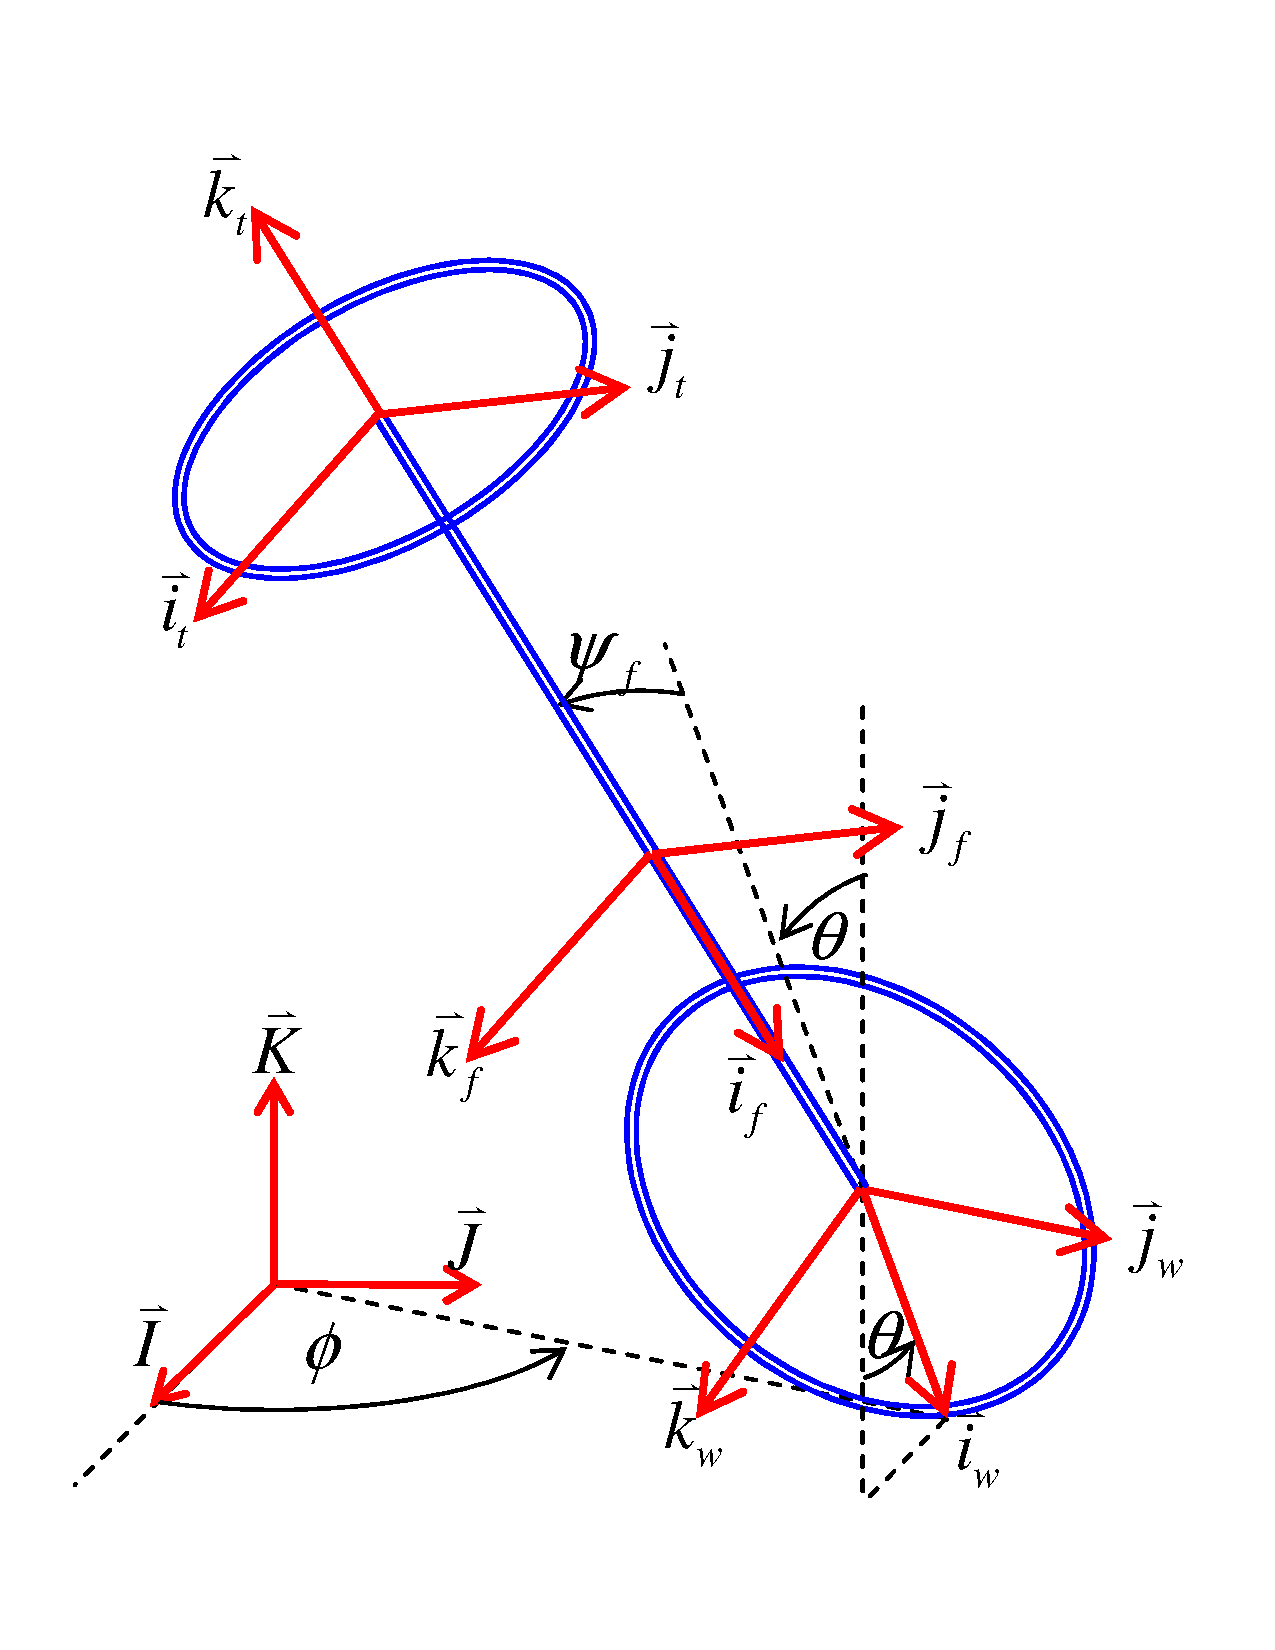
\includegraphics[height=8cm]{figures/angles.pdf}
    \end{center}
    \caption{Diagram showing Euler angles for the rotation of the unicycle
    (from \cite{ref:forster})}
    \label{fig:unicycle_angles}
    \end{figure}

However, this ignores the presence of unobserved states in the system like
delays, backlash in the gears, etc. To help the dynamics model deal with these
problems, we tried giving it access to the previous state and control input,
in effect modelling it as a 2$^\textrm{nd}$ order Markov chain:
\[
  \boldsymbol{q}_2[n] = \left[ \begin{array}{l}
    \boldsymbol{q}[n-1] \\
    \boldsymbol{u}[n-1] \\
    \boldsymbol{q}[n] \\
  \end{array} \right]
\]

This significantly improved the accuracy of the dynamics model, which in turn
suggests that unobserved states are significant in the behaviour of the real
unicycle. 

\subsubsection{Controller Form}

The most basic form of controller is a linear controller,
$\boldsymbol{g}(\boldsymbol{q}[n]) = \boldsymbol{W} \boldsymbol{q}[n] +
\boldsymbol{p}$, where $\boldsymbol{W}$ is a matrix of weights and
$\boldsymbol{p}$ is a vector of offsets. This form is capable of stabilising
the ideal inverted pendulum, and indeed proved sufficient to stabilise the 2D
system.

However, the linear controller cannot generate the correct turning command as
shown in Figure~\ref{fig:xor}---this is equivalent to the XOR problem, and can
be solved by using a quadratic controller. This takes the form:
\[
  g_i(\boldsymbol{q}[n]) = p_i + \sum_{j=1}^D w_{i,j} q_j[n] +
    \sum_{j=1}^D \sum_{k=j}^D h_{i,j,k} q_j[n] q_k[n]
\]
  
\begin{figure}[htbp]
  \begin{center}
    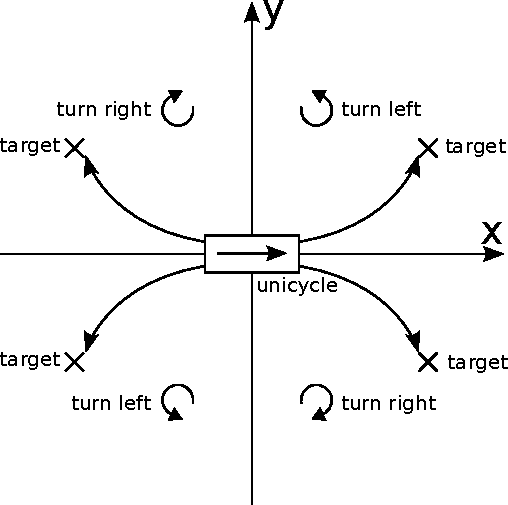
\includegraphics[width=8cm]{figures/xor.pdf}
    \end{center}
    \caption{Correct turning command in unicycle-centred coordinates}
    \label{fig:xor}
    \end{figure}

It was found that the controllers performed significantly better when using
$\boldsymbol{q}_2[n]$ as input, instead of $\boldsymbol{q}[n]$. To understand
this, consider the effect with a linear policy: the controller for the
augmented state is equivalent to a combination of a two-tap FIR filter and a
first-order IIR filter on the original state:
\begin{IEEEeqnarray*}{rCl}
  \boldsymbol{u}[n] &=& 
  \boldsymbol{g}(\boldsymbol{q}_2[n]) = \boldsymbol{W} \boldsymbol{q}_2[n] \\
   &=& \boldsymbol{W}_1 \boldsymbol{q}[n-1] + \boldsymbol{W}_2
   \boldsymbol{u}[n-1] + \boldsymbol{W}_3 \boldsymbol{q}[n]
  \end{IEEEeqnarray*}

This allows the RMLC system to create basic low or high-pass filters in
the controller, and this additional freedom improved the subjective quality of
the controllers trained.

\subsubsection{Loss Function}

The main concerns when choosing a loss function are accurately represent what
is desired of the controller, and to ensure that different desires are
appropriately weighted. When stabilising the ideal unicycle, Rasmussen was
successful using the following form of loss function:

\[
  1 - \mathcal{N}(\boldsymbol{q}[n]; \boldsymbol{\mu}, \boldsymbol{\Sigma})
  = 1 - \exp\left(\sum_{d=1}^D - \frac{(q_d[n] - \mu_d)^2}{w_d^2}\right)
\]

This is configured using $w_d$, the characteristic widths for each variable.
To ignore a variable, take $w_d^{-2} = 0$. While the RMLC system is not too
sensitive to these values, it is important to set them appropriately. During a
test run on the 2D system, we accidentally set the characteristic pitch angle
to $10^\circ$ and the characteristic distance (from the origin) to around
10cm. This meant that the preferred policy was to fall over immediately, to
prevent travelling away from the origin. Loosening the characteristic distance
to 30cm led to a controller that balanced the system.

For the ideal unicycle, Rasmussen chose to penalise the pitch and roll angles,
to encourage the system to keep the robot vertical.  In addition, he chose to
penalise the yaw rate $\dot{\phi}$ and flywheel rate $\dot{\psi}_t$ to prevent
the system from using a ``spinning-top'' like approach to balance, and to
penalise the distances from the origin, $x_c$ and $y_c$, to prevent the system
from driving the robot very fast to enhance stability.

We used the same loss function structure, with characteristic widths of
$9^\circ$ on the angles, 1 metre on the distances and 1 rps \& 3 rps on the
yaw \& flywheel rates respectively. Unlike the ideal unicycle, the real
unicycle has an upper limit on the flywheel speed, so the ``spinning-top''
strategy is not viable, so it is possible that the yaw \& flywheel rates need
not be penalised. This was not tested.

\subsubsection{Timestep}

The RMLC approach assumes a discrete-time system - to apply it to a continuous
time system, it must be discretised. We used a zero-order hold (ZOH) on the
control signal: $u(t)~=~u[\lfloor\frac{t}{T}\rfloor]$

Training for the ideal unicycle, Rasmussen found it desirable to choose the
largest timestep $T$ with which the system can be stabilised, to reduce the
computational cost of the optimisation, and to avoid problems with noise
buildup from many repeated applications of the transition function
$\boldsymbol{f}$. He chose a timestep of $\frac{1}{7}$ seconds.

However, for the real unicycle, both McHutchon and we found that the predicted
trajectories are more confident and reliable, and controllers perform better,
when using a timestep of $\frac{1}{20}$ seconds. It was hoped that this was
because the sensors were noisier in real life, and so a shorter time in the
ZOH led to several successive noisy control settings being averaged by the
low-pass effect of the system, reducing the effect of noise. However,
upgrading the sensors didn't seem to change this, so there is possibly another
cause.

\section{Hardware and Software}

When the project started, some of the requirements were already clear, as a
result of the previous work on the unicycle. As such, extensive changes to the
hardware and a complete rewrite of the controller software were required to
fix issues that had been turned up by the previous year's work, and to prepare
it for 3D balance. A brief summary of the changes is below, followed by
greater detail where necessary.

\begin{itemize}

  \item The cumbersome FPGA-based controller used previously was replaced with
    an Arduino microcontroller, allowing changes to be made faster and more
    easily.

  \item Older gyroscopes and very noisy angle sensors were replaced by modern
    MEMS gyroscopes and accelerometers.

  \item Algorithms for keeping track of angle and position in 3D were written.

  \item A new motor controller was built for the flywheel, as well as a
    quadrature encoder for speed sensing.

  \item A sensor for the battery voltage was added, to ensure it could supply
    sufficient power to the motors.

  \item We designed and tested a number of methods of protecting the unicycle
    from falling, while allowing 3D movement.

  \item Some faults were identified and could not be fixed, so tests and
    error-checking were added to ensure these did not corrupt the data.

  \item To improve safety, the motor is disabled when a user presses a switch
    on the chassis or when the unicycle nears the ground.

\end{itemize}

\begin{figure}[htpb]
  \begin{center}
    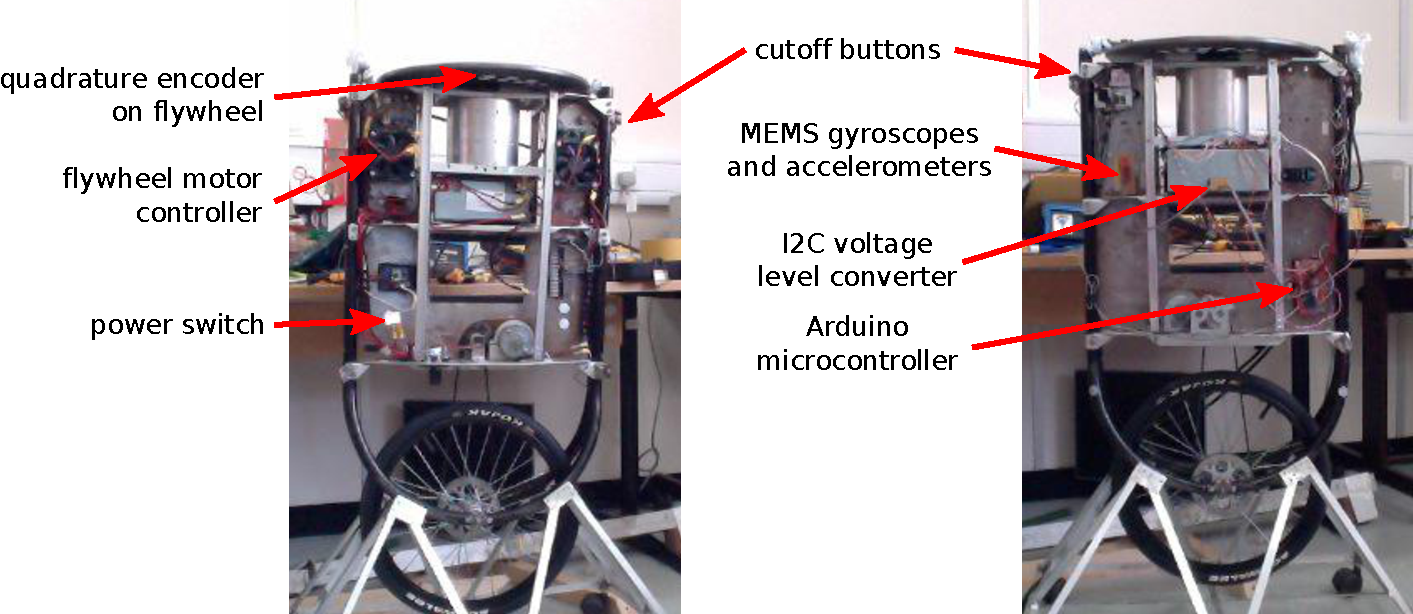
\includegraphics[width=15cm]{figures/hardware.pdf}
    \end{center}
    \caption{Summary of changes to unicycle hardware}
    \label{fig:hardware}
    \end{figure}

\subsection{Sensing}

\subsubsection{Angle Sensing}

The unicycle had previously used a MEMS rate gyroscope and a pair
of infra-red distance sensors to keep track of its angle. However, these were
reported to be extremely noisy, and were blamed for a large part of the poor
performance of the previous system. Our supervisor had already purchased the
ITG-3200, a 3-axis MEMS rate gyroscope with in-built temperature compensation
and low-pass filtering. We later purchased an ADXL345, a 3-axis MEMS
accelerometer, to determine the absolute angle of the unicycle.

The ITG-3200 rate gyro determines the angular velocity of the chip (and thus
the unicycle) around each of its 3 axes. These values are offset by some
unknown bias - this is determined before the trial by averaging the output
when stationary, and is assumed to be approximately constant during a trial.
They can then be converted to radians per second with a calibration factor
from the datasheet \cite{ref:itg3200}.

To keep track of the absolute angle, these angular velocities must be
integrated. There are 3 possible ways to keep track of rotations in 3D, of
which unit quaternions were chosen as best suited to the project.

\begin{description}
  \item[Euler angles]
    These are the yaw, roll and pitch angles shown in
    Figure~\ref{fig:unicycle_angles}. They are required for the controller,
    and so other forms must be converted to them. However, they suffer from
    gimbal lock---in certain positions, it is impossible to represent a
    small rotation with a small change in the Euler angles. They also require
    trigonometric functions in the integration loop: a problem for fast
    integration on embedded platforms.

  \item[Direction Cosine Matrices (DCMs)]
    A DCM is an orthonormal rotation matrix, representing the rotation from
    the global coordinate system to the body's coordinate system. They require
    only basic linear algebra to understand. However, when errors in
    integration accumulate, the matrix will no longer be orthonormal, and
    there is no clear way to fix this.

  \item[Unit quaternions]
    Quaternions extend the complex numbers into 3D. Just as a complex number
    of unit magnitude can represent a rotation in the 2D plane, a quaternion
    of unit magnitude can represent a rotation in 3D. Although they may appear
    confusing, they have the tightest integration loop, do not suffer from
    gimbal lock and can be normalised by simply dividing by the magnitude.

    \end{description}


\paragraph{Quaternion Integration}
Given the unit quaternion representing a rotation from the global coordinate
system to that of the unicycle, $\boldsymbol{q}[n] = q_w + q_x
\boldsymbol{i} + q_y \boldsymbol{j} + q_z \boldsymbol{k}$, and rate gyro
outputs $\omega_x$, $\omega_y$ and $\omega_z$, we can integrate
the angular velocities with $\boldsymbol{q}[n+1] = \boldsymbol{q}[n] \left(1 +
\frac{\omega_x \Delta t}{2} \boldsymbol{i} + 
\frac{\omega_y \Delta t}{2} \boldsymbol{j} + 
\frac{\omega_z \Delta t}{2} \boldsymbol{k}\right)$. For more details on this,
see \cite{ref:quaternions}.

\paragraph{Euler Angles of a Quaternion}
Unfortunately, the mechanical analysis of Forster (and thus the simulation of
the ideal unicycle) uses a different angle convention to all other sources
located. We chose to continue with this convention, and so the expressions for
converting a quaternion to Euler angles had to be rederived. Using a
convention of yaw around the vertical $y$-axis, roll around the forward
$x$-axis and pitch around the sideways $z$-axis (the axes of the mounted
gyroscope) we get:
\begin{IEEEeqnarray*}{rCl}
  \phi &=&  \tan^{-1}\left(\frac{2q_xq_y +
  2q_yq_w}{-q_x^2-q_y^2+q_z^2+q_w^2}\right) \\
  \theta &=&  \sin^{-1}\left(2q_wq_x - 2q_yq_z\right) \\
  \psi_f &=&  \tan^{-1}\left(\frac{2q_xq_y + 2q_zq_w}{-q_x^2+q_y^2-q_z^2+q_w^2}
  \right)\\
  \end{IEEEeqnarray*}

\paragraph{Angular Velocities}
To calculate the angular rates, $\dot{\phi}$, $\dot{\theta}$ and
$\dot{\psi}_f$, we convert the quaternion to a DCM, and then apply expressions
for the derivatives of the Euler angles of a DCM. This could cause a division
by zero in a gimbal lock situation, but fortunately the unicycle never reaches
such positions.
\begin{IEEEeqnarray*}{rCl}
  \left[\begin{array}{lll}
    d_{11} & d_{12} & d_{13} \\
    d_{21} & d_{22} & d_{23} \\
    d_{31} & d_{32} & d_{33} \\
    \end{array}\right] &=&
  \left[\begin{array}{lll}
    1-2q_y^2-2q_z^2 & 2q_xq_y-2q_zq_w & 2q_xq_z+2q_yq_w \\
    2q_xq_y+2q_zq_w & 1-2q_x^2-2q_z^2 & 2q_yq_z-2q_xq_w \\
    2q_xq_z-2q_yq_w & 2q_yq_z+2q_xq_w & 1-2q_x^2-2q_y^2 \\
    \end{array}\right] \\
  \dot{\phi} &=& \frac{(d_{12}d_{32}-d_{12}d_{33})\omega_x +
    (d_{11}d_{33}-d_{13}d_{31})\omega_y}{d_{13}^2 + d_{33}^2} \\
  \dot{\theta} &=& \frac{d_{22} \omega_x - d_{21}
    \omega_y}{\sqrt{1-d_{23}^2}} \\
  \dot{\psi}_f &=& -\frac{d_{23}(d_{21}\omega_x + d_{22}\omega_y)}{d_{21}^2 +
    d_{22}^2} + \omega_z
  \end{IEEEeqnarray*}

\paragraph{Initial Angle}
To determine the initial angle of the unicycle, we take an average
accelerometer reading while the unicycle is initially stable. This is a 3D
vector, representing the direction of gravity in the reference frame of the
rotated unicycle. By considering the DCM resulting from rotations in pitch and
roll, we can determine the pitch and roll angles, and use these to construct
an initial rotation quaternion.
\begin{IEEEeqnarray*}{rCl}
  \boldsymbol{D} &=&  \left[\begin{array}{lll}
    \cos \psi_f & -\sin\psi_f & 0 \\
    \cos \theta \sin \psi_f & \cos \theta \cos \psi_f & -\sin \theta \\
    \sin \theta \sin \psi_f & \sin \theta \cos \psi_f & \cos \theta 
    \end{array}\right] \\
  \left[\begin{array}{l}
    a_x \\ a_y \\ a_z
    \end{array}\right] &=& 
    \left[\begin{array}{l}
      \cos \theta \sin \psi_f \\ \cos \theta \cos \psi_f \\ -\sin \theta
      \end{array}\right]\\
  \theta &=&  -\sin^{-1}(a_z) \\
  \psi_f &=&  \tan^{-1}\left(\frac{a_x}{a_y}\right) \\
  \boldsymbol{q} &=&  \left(\cos\left(\frac{\theta}{2}\right) +
  \boldsymbol{i}\sin\left(\frac{\theta}{2}\right)\right)
  \left(\cos\left(\frac{\psi_f}{2}\right) +
  \boldsymbol{k}\sin\left(\frac{\psi_f}{2}\right)\right)
  \end{IEEEeqnarray*}

\paragraph{Gyro Noise and Drift}
The approach described above is vulnerable to drift: accumulating errors in
the integration of the gyroscope, especially when the zero-offset of the
gyroscope changes. To evaluate the effect of this, the gyro was sampled for 10
seconds when stationary. The rate readings are shown in
Figure~\ref{fig:gyro_stat}. It is clear that the noise and drift are on the
same order of magnitude, over a 10 second trial, the zero-offset changed by
about 0.1 deg s$^{-1}$, leading to a drift of below 1$^\circ$. This was judged
as acceptable.  If we wished to conduct longer trials, we could use one of a
variety of fusion methods such as state observers, Kalman filters, or one of
many highly tuned implementations developed by UAV hobbyists
\cite{ref:gluonpilot}.

\begin{figure}[htpb]
  \begin{center}
    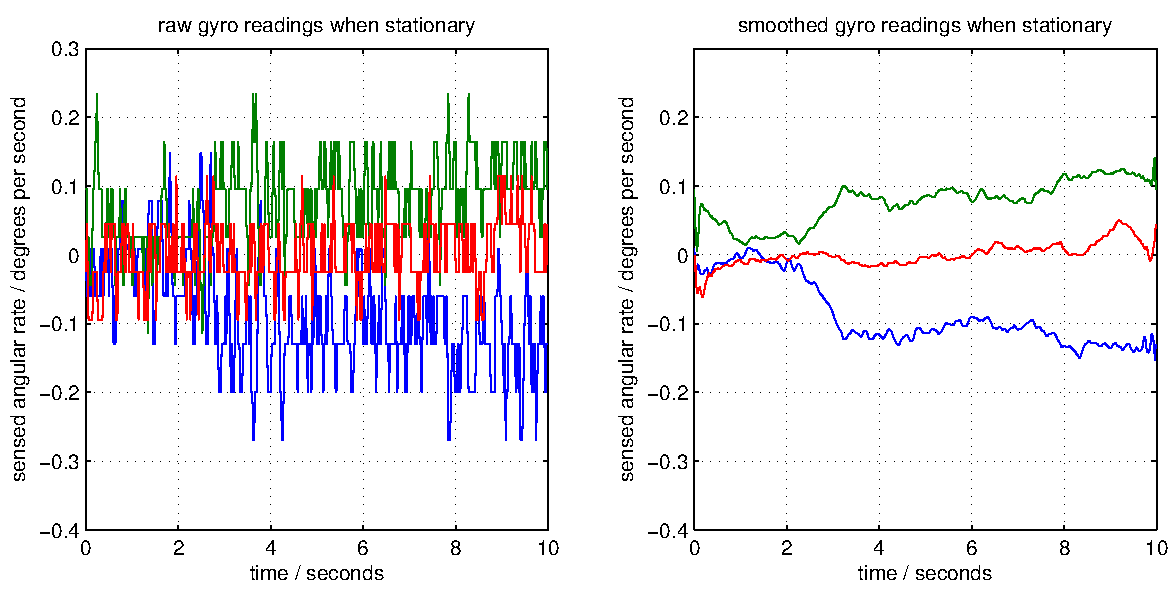
\includegraphics[width=13cm]{figures/gyro_stat.pdf}
    \end{center}
    \caption{Gyro readings when stationary}
    \label{fig:gyro_stat}
    \end{figure}

\paragraph{Accelerometer Noise}
Figure~\ref{fig:acc_stat} shows the accelerometer noise when stationary (the
mean reading has been subtracted). (Note that the noise characteristic is very
different for one axis compared to the other 2 - this is because this axis is
perpendicular to the chip, and is built differently.) This corresponds to
noise standard deviations for pitch and roll of about 0.5$^\circ$, but this
can be reduced by averaging many readings. More detail on the use of the
accelerometer can be found in Douglass's report.

\begin{figure}[htpb]
  \begin{center}
    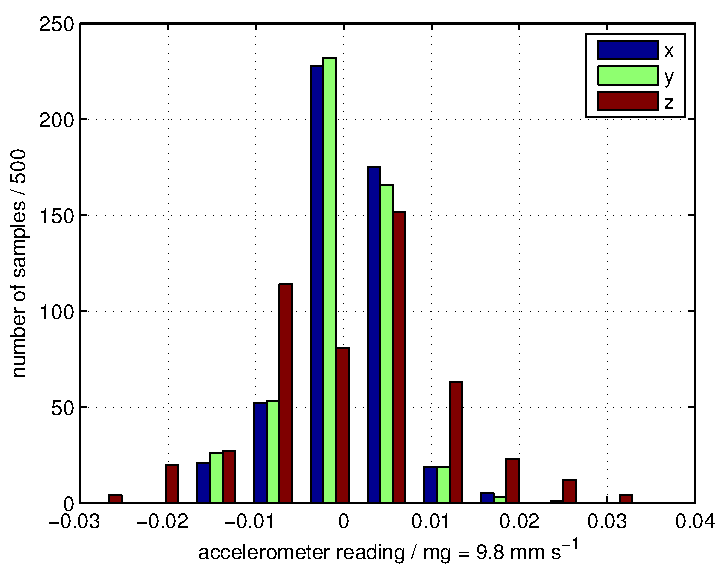
\includegraphics[height=7cm]{figures/acc_stat.pdf}
    \end{center}
    \caption{Accelerometer readings when stationary}
    \label{fig:acc_stat}
    \end{figure}

\subsubsection{Position Sensing}

In order to reduce the number of state variable necessary, Rasmussen used
self-centred coordinates to keep track of the position of the target. In
these coordinates, the unicycle is at (0, 0) and faces along the positive
$x$-axis, as shown in Figure~\ref{fig:xor}. At each timestep, we must use the
change in yaw angle $\Delta\phi$ and the change in wheel angle
$\Delta\psi_w$ (along with wheel radius $r_w$) to calculate the new target
position. From Figure~\ref{fig:scc} we can see that $x_c$ and $y_c$ must be
modified as follows:

\[
\begin{bmatrix}
  x_c[n+1] \\
  y_c[n+1]
\end{bmatrix} =
\begin{bmatrix}
  \cos(-\Delta\phi) & -\sin(-\Delta\phi) \\
  \sin(-\Delta\phi) & \cos(-\Delta\phi)
\end{bmatrix}
\begin{bmatrix}
  x_c[n] \\
  y_c[n]
\end{bmatrix} +
\begin{bmatrix}
  0 \\ -r_w\Delta \psi_f
\end{bmatrix}
\]

\begin{figure}[htpb]
  \begin{center}
    \def\svgwidth{15cm}
    \input{figures/scc.pdf_tex}
    \end{center}
    \caption{Effect of unicycle movement on target position in self-centred
    coordinates}
    \label{fig:scc}
    \end{figure}

The shaft encoder used to detect wheel angle changes has a quantisation error
of around 1mm. The buildup in yaw error over the trial should be less than
1$^\circ$, so when the distance from the target is around 1m, we can expect
errors of around $1\textrm{mm} + 1^\circ \cdot \frac{\pi}{180} \cdot
1\textrm{m} \approx 2$cm.  This should be more than accurate enough for the
application.

\subsubsection{Wheel Speed Sensing}

When we started the project, a quadrature encoder was being used to measure
the position and speed of the wheel. This is a digital sensor, which generates
a pulse every time the wheel moves through $\frac{1}{512}$ of a revolution.
Merely counting these pulses gives extremely good measurements of position
(accurate to around 1mm) but it is harder to measure speed. The approach being
used previously was to measure the number of pulses in 40ms, but this leads to
a quantisation error of 25 pulses per second, or 2.5cm s$^{-1}$.

More details on how the quadrature encoders are used to sense position can be
found in Douglass's report \nocite{ref:douglass}.

An alternative method is to measure the amount of time between the last two
pulses, but at high speeds this time may be very short, and this time may be
hard to measure accurately.

This became more important when we added a quadrature encoder for the
flywheel: the sensors used are much less accurate than those on the wheel.
There are only 72 pulses per revolution, and there is significant
non-uniformity around the wheel. This means that the first method would have a
quantisation error of 125$^\circ/$s, and the second method would only be
accurate to within around 50\%. This is unacceptable accuracy.

After reading a comparative analysis of various methods \cite{ref:encspeed},
we decided on a method that combines the benefits of the two approaches above.
It adapts the size of the 40ms window to contain an integer number of pulses,
eliminating quantisation error. At high speeds, it is similar to the first
scheme, considering the length of many pulses to reduce the effect on
non-uniformity and timing errors. At sufficiently low speeds, it adapts to
only using the most recent pulse, avoiding quantisation error.
Figure~\ref{fig:encoder_speed} explains how it works---note that some thought
is required about what should be returned when no pulses are observed in the
window.

\begin{figure}[htpb]
  \begin{center}
    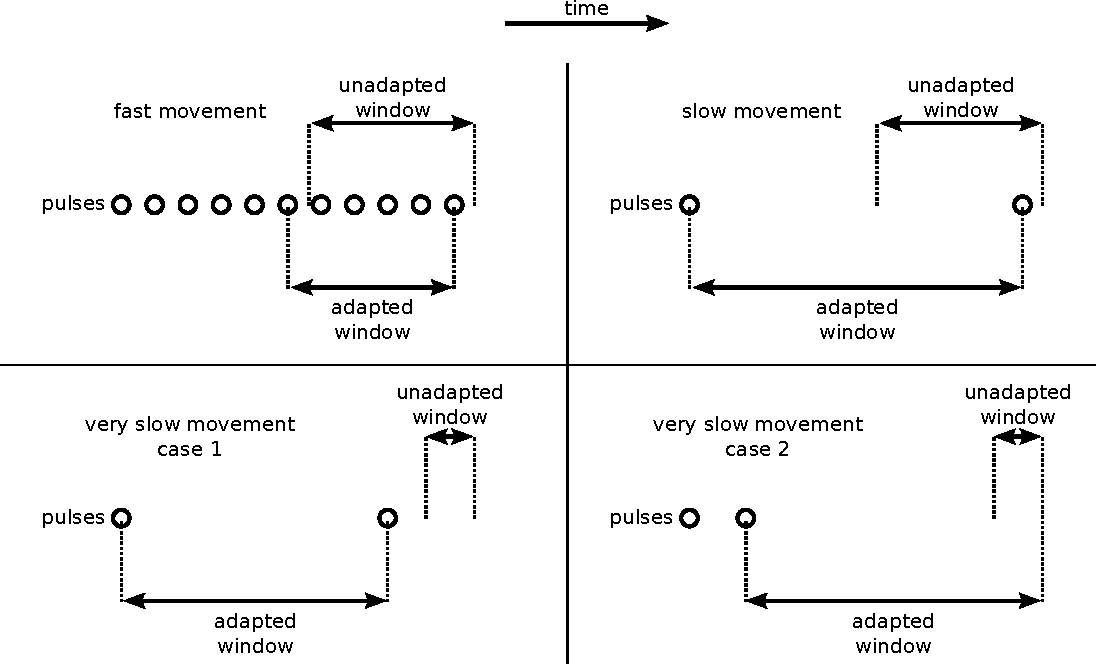
\includegraphics[width=15cm]{encoder_speed.pdf}
    \end{center}
    \caption{Adaptive-window encoder speed measurement}
    \label{fig:encoder_speed}
    \end{figure}

\subsection{Fall Protection}

Due to the trial-and-error nature of the RMLC method, the unicycle must be
able to survive using a controller that may be worse than none at all. When
the dynamics model is inaccurate, it may choose a controller than throws the
30kg unicycle towards the ground with all the force of a 240W motor.
Figure~\ref{fig:alu_bar} shows the effect of repeated trials on the aluminium
bar used in the previous year.

\begin{figure}[htpb]
  \begin{center}
    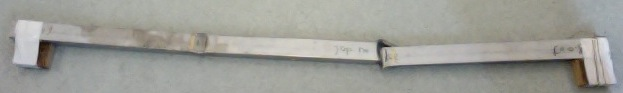
\includegraphics[width=15cm]{alu_bar.jpg}
    \end{center}
    \caption{Damaged aluminium box section from previous year's testing}
    \label{fig:alu_bar}
    \end{figure}

Two approaches had been used previously: suspending the unicycle from a crane
in the Structures Lab, and equipping the unicycle with a support structure
that hits the ground and stops the fall before it becomes dangerous.
Suspending the unicycle limits its range of motion, as if it travels too far
the rope will pull it over, as shown in Figure~\ref{fig:suspended}.

We suspected that the ability to travel freely would be important for the
unicycle, since if an RMLC system is unable to experience control policies
that travel a long way, the dynamics model will never learn that this can
happen and that it should try to avoid it. As such, we chose to build a wooden
skirt which would travel with the unicycle and protect it from falling, as
shown in Figure~\ref{fig:skirt}. More details on the design of the skirt,
including a CAD drawing of the mounted skirt, can be found in Douglass's
report.

\begin{figure}[htpb]
  \begin{center}
    \subfigure[Wooden skirt]{
      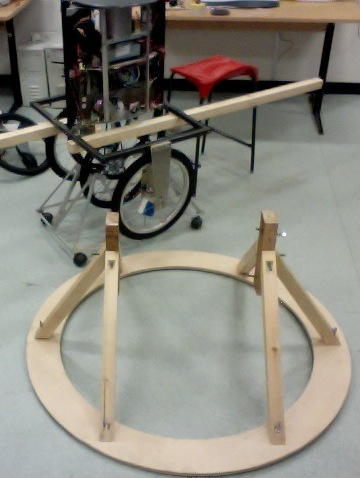
\includegraphics[height=6cm]{skirt.jpg}
      \label{fig:skirt}
    }
    \subfigure[Suspended unicycle]{
      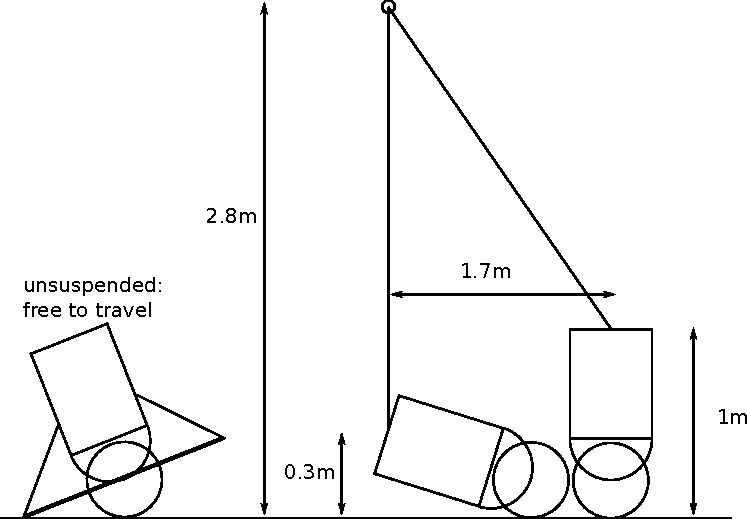
\includegraphics[height=6cm]{suspended.pdf}
      \label{fig:suspended}
    }
    \end{center}
    \caption{Unicycle fall protection methods}
    \label{fig:fall_protection}
    \end{figure}

\subsection{Inability to Spin}

After building the skirt and preparing the necessary hardware and software, we
started training the unicycle. However, it made very little progress, and
would consistently seem to fall to the side, without turning in that direction
and driving forwards to pick itself up. We tried modifying the controller to
send the maximum motor command to the flywheel at all times, and found that it
could only turn around 30$^\circ$ before falling.

It is very important that the robot be able to turn sufficiently fast to be
able to point in the direction in which it is falling, before it has fallen.
We considered various possible causes for the slow turning:

\begin{itemize}
  \item Adding the skirt had increased the moment of inertia, making it spin
    slowly.
  \item Friction with the ground was causing it to turn too slowly.
  \item The gear ratio for the flywheel was chosen badly.
  \item The flywheel had insufficient moment of inertia to turn the robot fast
    enough, even without the above effects.
  \item The flywheel motor was insufficiently powerful, even without the above
    effects.
    \end{itemize}

To try to quantise this, we suspended the robot above the ground, and tested
the response of the system to a step increase in flywheel command. We then
used a mathematical model to quantify how changing various variables would
affect the spin speed.

\subsubsection{Spin Analysis}

The response of a DC motor can be well modelled as \cite{ref:6302}:

\begin{equation*}
  \frac{\Omega_\textrm{motor}(s)}{V(s)} = \frac{K_t}{(R+Ls)(Js+b)+K_t^2}
  \end{equation*}

where we define

\begin{description}
  \item[$\omega$] Speed of motor shaft
  \item[$V$] Motor input voltage
  \item[$K_t$] Motor torque constant
  \item[$R$] Motor armature resistance
  \item[$L$] Motor armature inductance (usually negligible)
  \item[$J$] Moment of inertia of object on motor shaft
  \item[$b$] Damping on motor shaft (sometimes negligible)
    \end{description}

The effect of the gear train is analogous to that of a transformer: the
flywheel MoI, $J_f$ appears to the motor as an MoI of $J = \frac{J_f}{n^2}$.
More obviously, it has the effect that $\omega_\textrm{flywheel} =
\frac{\omega_\textrm{motor}}{n}$.

So, neglecting $L$ and $b$, we have:
\begin{IEEEeqnarray*}{rCl}
  \frac{\Omega_\textrm{flywheel}(s)}{V(s)} &=& 
     \frac{K_t}{R \frac{J_f}{n^2} s+K_t^2} \\
    &=& n^{-1} K_t^{-1} \frac{1}{\frac{R J_f}{n^2 K_t^2} s + 1} \\
  \end{IEEEeqnarray*}

The corresponding step response is of the form:
\[
  \omega_\textrm{flywheel}(t) = K (1 - e^{-\frac{t}{\tau}})
\]

Fitting this to the observed step response, as in Figure~\ref{fig:step}, tells
us that $K = 33$ and $\tau = 0.55$ seconds.

If we integrate to get the flywheel angle, and then assume that there are no
external torques on the robot and that the robot has MoI $J_r$:
\begin{IEEEeqnarray*}{rCl}
  \omega_\textrm{flywheel}(t) &=& K (1 - e^{-\frac{t}{\tau}}) \\
  \theta_\textrm{flywheel}(t) &=& K (t + \tau (e^{-\frac{t}{\tau}} - 1)) \\
  \theta_\textrm{robot}(t) &=& \frac{J_f}{J_r} K (t + \tau (e^{-\frac{t}{\tau}} - 1)) \\
  \end{IEEEeqnarray*}

\begin{figure}[htbp]
  \begin{center}
    \subfigure[Flywheel speed]{
      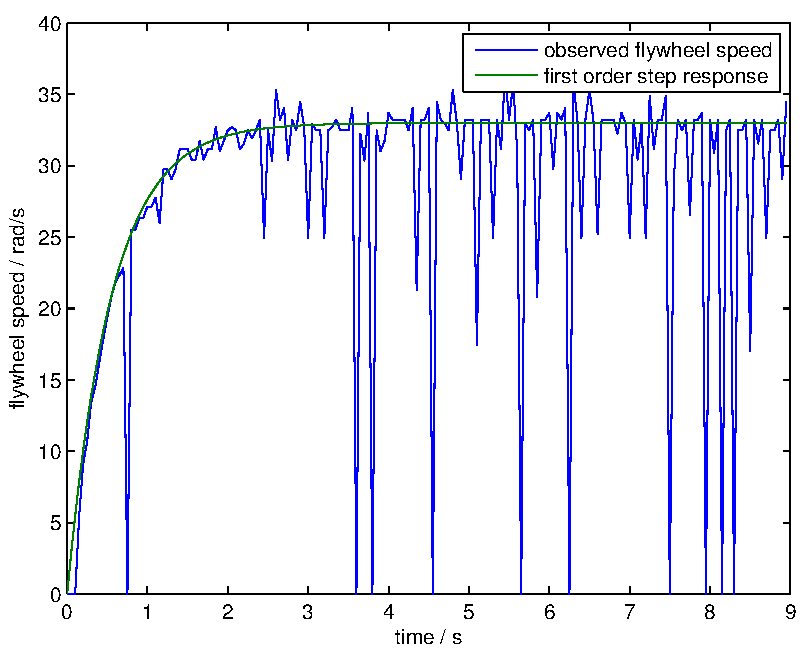
\includegraphics[height=6cm]{step.pdf}
      \label{fig:step}
    }
    \subfigure[Robot angle]{
      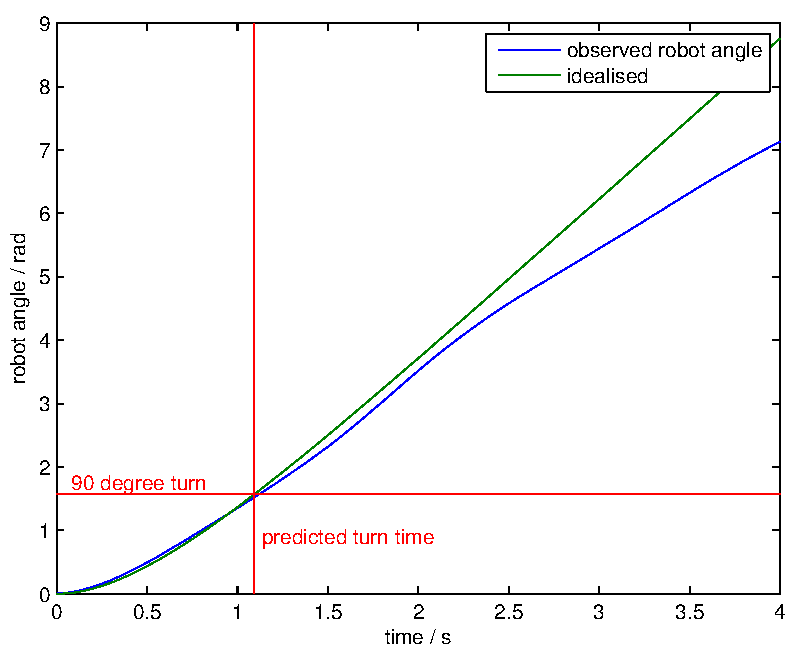
\includegraphics[height=6cm]{step_angle.pdf}
      \label{fig:step_angle}
    }
    \end{center}
    \caption{Response to step in flywheel command}
    \end{figure}

By fitting (see Figure~\ref{fig:step_angle}) we get $\frac{J_r}{J_f} = 13$
(including the skirt). As the angle increased, the rope supporting the
unicycle twisted, slowing the robot's spin, but the initial fit is good.  We
can now solve for the time to turn 90$^\circ$. This model predicts a turn time
of 1.1 seconds for the suspended robot: this is far too slow, and so clearly
contact with the ground is not entirely to blame---we must look elsewhere to
solve the problem.

We can check the observed value of $\frac{J_r}{J_f}$ by estimating the moments
of inertia. Modelling the flywheel as a uniform disc of mass 8kg, the robot as
a uniform cuboid of mass 24kg, and the skirt as mass concentrated at 55cm (the
ring) and 40cm (the struts) from the body:
\begin{IEEEeqnarray*}{rCl}
  J_f &=& \frac{1}{2}M R^2
    = \frac{1}{2} \cdot 8 \cdot (0.2)^2 \\
    &=&  0.16 \textrm{ kg m}^2 \\
  J_r &=& \frac{1}{12}M L^2
    = \frac{1}{12} \cdot 24 \cdot (0.4)^2\\
    &=&  0.32\textrm{ kg m}^2 \\
  \textrm{mass of skirt} &=& 4.4 \textrm{ kg} \\
  \textrm{mass of structs} &=& 3.5 \textrm{ kg} \\
  J_\textrm{skirt} &=& 3.5 \cdot 0.4^2 + 4.4 \cdot 0.55^2 \\
    &=&  1.89 \textrm{ kg m}^2\\
  \frac{J_r}{J_f} &=& 2\\
  \frac{J_r + J_\textrm{skirt}}{J_f} &=& 13.8\\
  \end{IEEEeqnarray*}

This backs up the result of the previous analysis, which suggested $\frac{J_r
+ J_\textrm{skirt}}{J_f} = 13$. With this model, we can predict the effect on
the turn time of various changes to the suspended
robot---Table~\ref{tab:turn_time} shows various possibilities, and makes it
clear that reducing or removing the skirt is most valuable improvement to
make.

\begin{table}[htbp]
  \centering
    \begin{tabular}{l l l | l}

      gear ratio & flywheel MoI & robot MoI & turn time \\
      \hline
      1x & 1x & 1x & 1.09s \\
      1x & 2x & 1x & 0.94s \\
      1.6x (optimum) & 2x & 1x & 0.87s \\
      1x & 10x & 1x & 0.85s \\
      4.8x (optimum) & 10x & 1x & 0.51s \\
      1x & 1x & $\frac{3.6}{13}$x (lightweight skirt) & 0.50s \\
      1x & 1x & $\frac{2}{13}$x (removed skirt) & 0.36s \\

    \end{tabular}
    \label{tab:turn_time}
    \caption{Ideal turn time under various conditions}
    \end{table}

\subsubsection{Solving the Spin Problem}

Having realised this, we redesigned the skirt to reduce its MoI. We reduced
the width of the rim from 12cm to 2cm, and replaced the wooden struts with
aluminium members. This reduced the MoI of the skirt by a factor of 7x, and
could still support the weight of the unicycle. However, after a few falls,
the wood had started to crack and one of the aluminium struts broke at the
joint. Despite reinforcing the wood with glue and aluminium struts, we were
unable to reach a design for the skirt that was both sturdy and light.

\begin{figure}[htpb]
  \begin{center}
    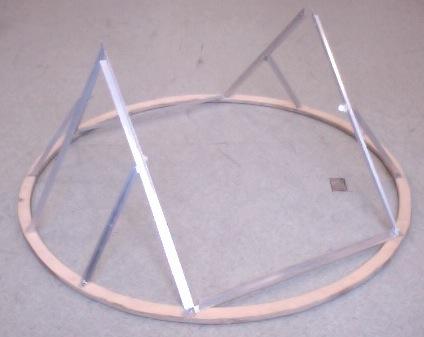
\includegraphics[width=7cm]{light_skirt.jpg}
    \end{center}
    \caption{Reduced-weight skirt}
    \label{fig:light_skirt}
    \end{figure}

Eventually, we chose to use a rope tied to the mezzanine in the foyer of the
Engineering department. This is a very busy area, and so testing can only be
done outside of the department's normal opening hours, but at least the
problematic effects of the skirt are completely removed.

\subsection{Known Issues}

Throughout the design process we found some problems with the unicycle's
hardware and software that we were unable to fix. When this occurred, we did
our best to stop them from interfering with the testing process.

\subsubsection{Toothed Belt}

The robot uses a toothed belt to transfer torque to the wheel, shown in
Figure~\ref{fig:fan_belt}. During tests, it would frequently slip when the
controller demanded large changes in motor velocity. This leads to a mismatch
between the encoder reading at the actual position, which would cause great
problems for the dynamic model. As such, it was critical to make sure that we
observed carefully for trials in which the belt slipped, and removed the
corrupted data from the logs. Towards the end of the testing process, we
installed an extra strut, also shown in Figure~\ref{fig:fan_belt} to maintain
tension in the belt.

\begin{figure}[htpb]
  \begin{center}
    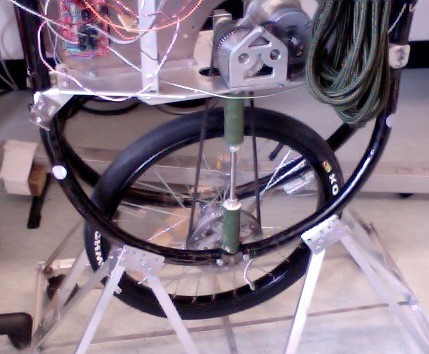
\includegraphics[width=6cm]{fan_belt.jpg}
    \end{center}
    \caption{Toothed belt and tensioning strut}
    \label{fig:fan_belt}
    \end{figure}

\subsubsection{Motor Control}

Unpredictably, one or both of the motors would fail move at all. This proved
extremely hard to debug, since sometimes even touching the circuit with a
single probe of a voltmeter would cause them to start working again. At one
time, we were able to investigate the problem with an oscilloscope---it
appeared that the inputs to the motor controller were behaving correctly, and
that while the PWM input went through to the output, both terminals of the
motor were driven with exactly the same PWM signal, with no potential
difference across the motor.

The cause of this is unknown, but likely an electrical problem due to the
unpredictable behaviour and sensitivity to contact from the voltmeter probe.
Because we were unable to prevent it from happening, we modified the software
to test both motors before every trial. This allowed us to power cycle the
system to avoid the problem.

\subsubsection{Flywheel Encoder}

The flywheel encoder is prone to generating spurious pulses---these can
manifest as sudden changes in direction, which are perceived as sudden stops
by the speed-sensing algorithm described earlier.
Figure~\ref{fig:bad_fly_speed} shows the effect of these spurious
transmissions---clearly extremely severe, and very problematic for the dynamic
model to predict.

\begin{figure}[htpb]
  \begin{center}
    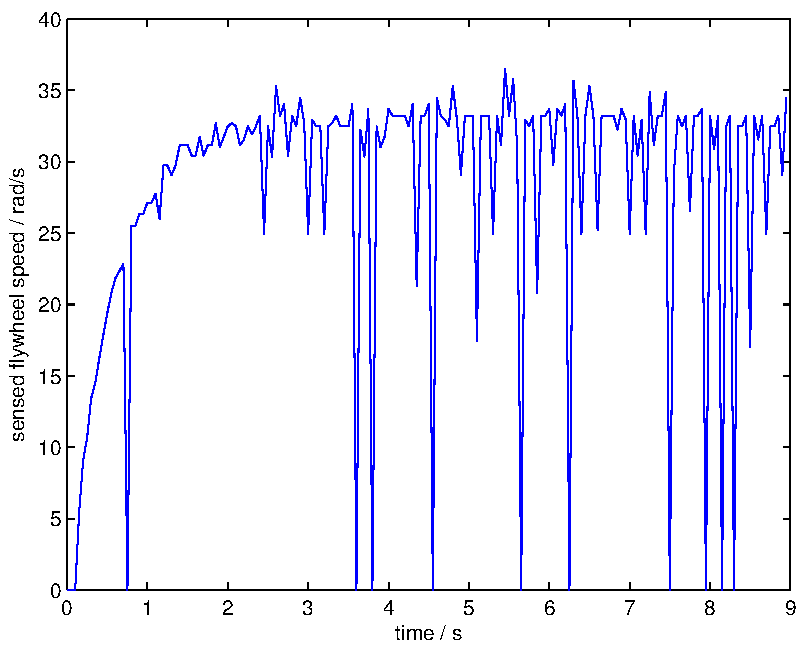
\includegraphics[height=7cm]{bad_fly_speed.pdf}
    \end{center}
    \caption{Corrupted flywheel speed measurements}
    \label{fig:bad_fly_speed}
    \end{figure}

As described in Douglass's report, the flywheel encoder uses Schmitt triggers
to digitise the analog encoder outputs. Figure~\ref{fig:scope_trace} shows a
trace of the input and output to this signal cleaning circuit (the two traces
have been traced in an image editor for clarity). There appears to be a
negative spike in the signal, part-way through the high cycle.  This is due to
interference between the two quadrature sensors (covering one emitter removed
the spike). Unfortunately, the low hysteresis voltage on the model of Schmitt
trigger used (0.4V min., 0.7V typ.) means that this is enough to reach the
threshold and cause problems. The extent of this problem was limited slightly
by placing a larger piece of cardboard between the two sensors.

\begin{figure}[htpb]
  \begin{center}
    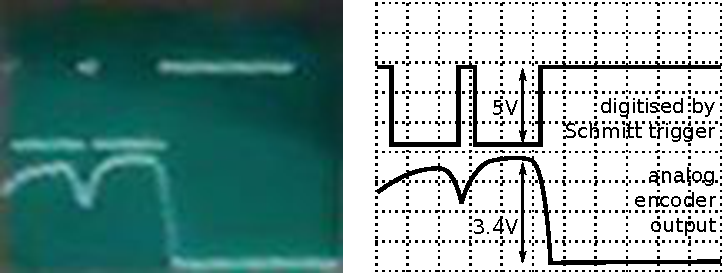
\includegraphics[width=13cm]{scope_trace.pdf}
    \end{center}
    \caption{Oscilloscope trace of flywheel encoder outputs}
    \label{fig:scope_trace}
    \end{figure}

The other problem visible is that the range of the analog signal is not 0--5V,
but around 0--3.4V. This is because the photodiode in the sensor is not fully
conducting when pointed at a white part of the pattern. To ensure that the
Schmitt trigger acted properly, we reduced its supply voltage to 3.3V. While
this meant that the input exceeded the supply voltage, and that the high-level
output was 3.3V, yet the AVR (the processor on the Arduino) operates on 5V,
both the Schmitt trigger \cite{ref:4093} and the AVR's \cite{ref:atmega}
datasheets stated that these were acceptable. This does have the effect of
further reducing the hysteresis voltage, but combined with the added
occlusion, it helped control the problem.

Despite these changes, the problem is still very sensitive to the orientation
of the sensors, and the shocks undergone during trials can cause it to
resurface. To avoid this, we adapted the software to try to test for this
problem before every trial, and we carefully inspected the logs after the
trials, in an attempt to detect signs of corrupted data.

\section{Results and Discussion}

\section{Conclusions}

\bibliography{iibproject}
\bibliographystyle{unsrt}

\pagebreak
\appendix

\section{Extra Stuff}

\end{document}
